\section{Geometria del piano}

\subsection{Angoli}

\begin{questions}
%%%%%%%%%%%%%%%%%%%%%%%%%%%%%%%%%%%%%%%%%%%%%%%%%%%%%%%%%%%%%%%%%
\question
\exonly{
Convertire in forma sessagesimale:
}

\begin{parts}
\part
\exonly{\ang{5,645}}  \solonly{\ang{5;38;42}}

\part
\exonly{\ang{15,37}}  \solonly{\ang{15;22;12}}

\part
\exonly{\ang{8,8}}  \solonly{\ang{8;48;}}
\end{parts}

%%%%%%%%%%%%%%%%%%%%%%%%%%%%%%%%%%%%%%%%%%%%%%%%%%%%%%%%%%%%%%%%%
\question
\exonly{

Convertire in gradi (forma decimale):
}

\begin{parts}
\part
\exonly{\ang{4;47;8} } \solonly{\ang{4.786}}

\part
\exonly{\ang{;895;}}  \solonly{\ang{14.92}}

\part
\exonly{\ang{12;38;24}}  \solonly{\ang{12.64}}
\end{parts}

%%%%%%%%%%%%%%%%%%%%%%%%%%%%%%%%%%%%%%%%%%%%%%%%%%%%%%%%%%%%%%%%%

\question
\exonly{

Convertire in gradi (forma decimale):
}

\begin{parts}
\part
\exonly{$\dfrac{\pi}{2}$} \solonly{\ang{90}}

\part
\exonly{$\dfrac{2}{3}\pi$}  \solonly{\ang{120}}

\part
\exonly{$\dfrac{5}{3}\pi$}  \solonly{\ang{300}}
\end{parts}

%%%%%%%%%%%%%%%%%%%%%%%%%%%%%%%%%%%%%%%%%%%%%%%%%%%%%%%%%%%%%%%%%

\question
\exonly{

Convertire in radianti (valore esatto):
}

\begin{parts}
\part
\exonly{\ang{30} } \solonly{$\dfrac{\pi}{6}$}

\part
\exonly{\ang{135}}  \solonly{$\dfrac{3}{4}\pi$}

\end{parts}

%%%%%%%%%%%%%%%%%%%%%%%%%%%%%%%%%%%%%%%%%%%%%%%%%%%%%%%%%%%%%%%%%

\question
\exonly{
	Calcolare l'angolo $\epsilon$ tra l'altezza $BH$ e la bisettrice $BI$ del vertice $B$.
}

\begin{parts}
\part
\exonly{
Nel caso particolare dove  $\angle ABC = 60^\circ$ e $\angle BCA= 40{}^\circ$.}
\solonly{$\epsilon=\ang{20}$}
\part
\exonly{In generale in funzione di  $\angle ABC = \alpha$ e $\angle BCA= \beta$ }
\solonly{$\epsilon=90 -\frac{\alpha}{2}-\beta$}
\end{parts}


\exonly{
\begin{tikzpicture}[line cap=round,line join=round,>=triangle 45,x=1.0cm,y=1.0cm,rotate=-30]
\draw (-1.0,3.0) node[left] {B}-- (3.0,3.0);
\draw (3.0,3.0) node[below right] {H}-- (3.0,0.0) ;
\draw (3.0,0.0) node[below] {A}-- (-1.0,3.0);
\draw (3.0,4.0)-- (-1.0,3.0);
\draw (3.0,4.0)-- (3.0,3.0);
\draw (3.0,6.0) node[right] {C}-- (3.0,4.0) node[below right] {I};
\draw (3.0,6.0)-- (-1.0,3.0) ;
\draw (2.8,3)--(2.8,3.2)--(3,3.2);
\draw (0,3) arc (0:14.04:1) node[right,midway,yshift=-0.1cm] {$\epsilon$} ;
\end{tikzpicture}
}

%%%%%%%%%%%%%%%%%%%%%%%%%%%%%%%%%%%%%%%%%%%%%%%%%%%%%%%%%%%%%%%%%%
%\question
%\exonly{
%\FR{
%Calculer les trois angles d`un triangle sachant que $2\cdot\alpha = \beta = \gamma$.
%}
%\DE{
%
%}}
%
%\solonly{$\alpha=\ang{36}$ \quad $\beta=\gamma=\ang{72}$
%}


%%%%%%%%%%%%%%%%%%%%%%%%%%%%%%%%%%%%%%%%%%%%%%%%%%%%%%%%%%%%%%%%%
\exnewpage
\question
\exonly{
Calcolare gli angoli $\gamma$ e $\delta$  in funzione di $\alpha$ e $\beta$:
%Calculer les angles $\gamma$ et $\delta$ en fonction de $\alpha$ et $\beta$ :
}

\begin{parts}
\part \exonly{
	se $ \alpha = 20^\circ$  e  $ \beta = 40^\circ$.}
\solonly{$\gamma=\ang{30}$ \quad  $\delta=\ang{30}$
}
\part \exonly{per $\alpha$ e $\beta$ qualunque.}
\solonly{$\gamma=\delta=90-\alpha -\beta$
}
\end{parts} 


%TODO : convert in TikZ
\includegraphics*[width=0.5\linewidth]{ch1-ex3}





%%%%%%%%%%%%%%%%%%%%%%%%%%%%%%%%%%%%%%%%%%%%%%%%%%%%%%%%%%%%%%%%%
%\question
%\exonly{
%\FR{
%Calculer les angles $\varphi_1$ à $\varphi_5$ si :
%$\alpha= 34^\circ$  et   $\delta = 60^\circ$.
%}
%\DE{
%
%}
%
%\includegraphics*[width=\linewidth]{ch1-ex4}
%}
%
%\solonly{
%$\varphi_1=\ang{124}$ \quad 
%$\varphi_2=\ang{112}$ \quad 
%$\varphi_3=\ang{128}$ \quad  \\
%$\varphi_4=\ang{142}$ \quad 
%$\varphi_5=\ang{68}$
%}



%%%%%%%%%%%%%%%%%%%%%%%%%%%%%%%%%%%%%%%%%%%%%%%%%%%%%%%%%%%%%%%%%

%\question
%\exonly{
%\FR{
%Calculer $\varphi$ à partir de $\alpha$:
%}
%\DE{
%
%}
%
%\includegraphics*[width=\linewidth]{ch1-ex5}
%}
%
%
%
%\begin{parts}
%\part
%\exonly{
%\FR{
%	pour $\alpha = \ang{36}$ 
%}
%\DE{
%	
%}}
%
%\solonly{$\varphi=\ang{117}$}
%
%
%\part
%\exonly{
%\FR{
%	pour un angle $\alpha$ quelconque
%}
%\DE{
%	
%}}
%
%\solonly{$\varphi=\ang{135} -\dfrac{\alpha}{2}$}
%
%
%\end{parts}




\end{questions}

%\exnewpage
%\subfile{../ch/5_2-Triangles_Semblables}
\subsection{Triangoli simili}
%\DE{\subsection{Änliches Dreiecks}}

\begin{questions}



%%%%%%%%%%%%%%%%%%%%%%%%%%%%%%%%%%%%%%%%%%%%%%%%%%%%%%%%%%%%%%%%%%%%%%%%
\question
\exonly{
Calcolare le misure mancanti $a$, $b$, $c$, $d$, $x$ e $y$ (in $\SI{}{\centi\meter}$) nei casi seguenti. Le rette $f$ e $g$ sono parallele.
}

%TODO : convert in TikZ
\exonly{\includegraphics*[width=0.5\linewidth]{ch2-ex3-1}}

\begin{parts}
\part 
\exonly{$a=\num{4.5}$ \quad $b=?$ \quad $c=3$  \quad  $d=2$ \\ $x=3$ \quad $y=?$}
\solonly{$b=3$ \quad $y=5$}

\part 
\exonly{$a=\num{6}$ \quad $b=?$ \quad $c=?$  \quad  $d=\num{1.6}$ \\ $x=5$ \quad $y=7$}
\solonly{$b=\num{2.4}$ \quad $c=4$}

\part 
\exonly{$a=?$ \quad $b=\num{4.2}$ \quad $c=\num{6.8}$  \quad  $d=\num{5.1}$ \\ $x=?$ \quad $y=\num{6.4}$}
\solonly{$a=\num{5.6}$ \quad $x=\num{3.66}$}

\part

\exonly{ $a=?$ \quad $b=\num{5.2}$ \quad $c=\num{2.8}$  \quad  $d=?$ \\ $x=\num{4.2}$ \quad $y=\num{8.1}$}
\solonly{$a=\num{5.6}$\quad $d=\num{2.6}$}

\part 
\exonly{$a=2$ \quad $b=\frac{7}{3}$ \quad $c=\frac{3}{2}$  \quad  $d=?$ \\ $x=\frac{6}{5}$ \quad $y=?$}
\solonly{$d=\frac{7}{4}=\num{1.75}$ \quad$y=\frac{13}{5}=\num{2.6}$}

\end{parts}


%%%%%%%%%%%%%%%%%%%%%%%%%%%%%%%%%%%%%%%%%%%%%%%%%%%%%%%%%%%%%%%%%%%%%%%%

%\question
%\exonly{
%\FR{Montrer que les triangles $ACB$ et $ADE$ sont semblables.
%
%Calculer $AD$ et $ED$ sans utiliser le théorème de Pythagore.
%
%$AB = 4$ ~ $BC = 3$ ~$AC = 5$ ~ $AE = 2$
%}
%}
%\exonly{\includegraphics*[width=0.6\linewidth]{ch2-ex1}}
%
%\solonly{$AD=\num{2.5}$ $ED=\num{1.5}$}

%%%%%%%%%%%%%%%%%%%%%%%%%%%%%%%%%%%%%%%%%%%%%%%%%%%%%%%%%%%%%%%%%%%%%%%%

\exnewpage
\question
\exonly{
A causa del lago non é possibile misurare la distanza $AC$.
Per poter calcolare questa distanza determiniamo i punti $B_1$ e $C_1$ tali per cui $B_1C_1$ sia parallela a $BC$.

Possiamo quindi misurare:   

$AB_{1}=\SI{15}{\meter}$ ~ $AC_{1}= \SI{9}{\meter}$ ~ $BB_{1}= \SI{133}{\meter}$.

Calcolare la distanza  $AC$.

}
\solonly{$AC=\SI{88.8}{\meter}$}

%TODO : convert in TikZ
\exonly{\includegraphics*[width=0.5\linewidth]{ch2-ex2}}


%%%%%%%%%%%%%%%%%%%%%%%%%%%%%%%%%%%%%%%%%%%%%%%%%%%%%%%%%%%%%%%%%%%%%%%%
%\question
%\exonly{
%\FR{
%Les diagonales d'un trapèze $ABCD$ se coupent en $O$.
%
%Calculer $OA$ sachant que les bases mesurent $AB = \SI{9}{\centi\meter}$ et $CD = \SI{6}{\centi\meter}$ et la diagonale $AC = \SI{10}{\centi\meter}$.
%}}
%
%\solonly{$OA=\SI{6}{\centi\meter}$}


%

%%%%%%%%%%%%%%%%%%%%%%%%%%%%%%%%%%%%%%%%%%%%%%%%%%%%%%%%%%%%%%%%%%%%%%%%
%\question
%\exonly{
%\FR{
%Quatre parallèles coupent deux droites sécantes $AC$ et $BD$.}}
%
%\begin{parts}
%\part
%\exonly{
%\FR{
%	Calculer $DF$ et $FH$ sachant que :
%	
%	$AC = 3$ ~$CE = 9$~ $EG = 6$ ~ $BD = 4$
%}} 
%\solonly{$DF=12$ \quad $FH=8$}
%
%\part
%\exonly{
%\FR{
%	Calculer $BD$ et $DF$ sachant que :
%	
%	$AC = 6$ ~$CE = 8$ ~$EG = 8$ ~ $BH = 33$
%}}
%
%\solonly{$BD=9$ \quad $DF=12$}
%\end{parts}
%
%
%\exonly{\includegraphics*[width=\linewidth]{ch2-ex5}}


%%%%%%%%%%%%%%%%%%%%%%%%%%%%%%%%%%%%%%%%%%%%%%%%%%%%%%%%%%%%%%%%%%%%%%%%
%\question
%\exonly{
%\FR{
%$f$, $g$ et $h$ sont trois droites parallèles.
%
%Calculer $AB$ et $CD$ lorsque $SB = \SI{7}{\centi\meter}$.
%}}
%
%
%\exonly{\includegraphics*[width=\linewidth]{ch2-ex6}}
%
%\solonly{$AB=\SI{5.6}{\centi\meter}$ \quad $CD=\SI{6}{\centi\meter}$k
%%%%%%%%%%%%%%%%%%%%%%%%%%%%%%%%%%%%%%%%%%%%%%%%%%%%%%%%%%%%%%%%%%%%%%%%%
%\exonly{\columnbreak}

%%%%%%%%%%%%%%%%%%%%%%%%%%%%%%%%%%%%%%%%%%%%%%%%%%%%%%%%%%%%%%%%%%%%%%%%

\question
\exonly{
Per determinare l'altezza di un palazzo un uomo si posiziona in modo da vedere la cima di un palo allineata alla cima del palazzo (altezza degli occhi  $\approx \SI{1.65}{\meter}$).

La distanza tra il palo (di altezza $\SI{3}{\meter}$) e il palazzo é di $\SI{33}{\meter}$ e quella tra il palo e la persone é di $\SI{7}{\meter}$


Calcolare l'altezza $h$ del palazzo.
}

\exonly{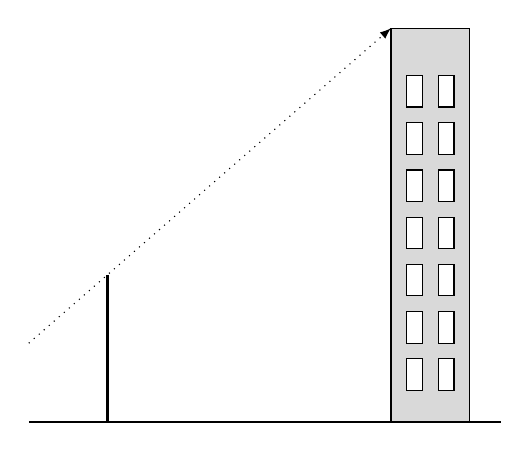
\begin{tikzpicture}
\human[0.5]{A}{0,0.5}
\draw[thick] (0,0) --(6,0);
\filldraw[fill=gray!30] (4.6,0) rectangle (5.6,5);
\draw[very thick] (1,0) -- (1,1.87);
%\draw[dotted,latex-latex] (0,1) -- node[above, midway] {\num{23.5}} (4.6,1);
\foreach \x in {0.2,0.8,1.4,2,2.6,3.2,3.8}
{
\filldraw[fill=white] (4.8, \x + 0.2) rectangle +(0.2,0.4) (5.2,0.2 + \x) rectangle +(0.2,0.4) ;
}
\draw[dotted,-latex] (0,1) -- (4.6,5);


\end{tikzpicture}}
%\exonly{\includegraphics*[width=\linewidth]{ch2-ex7}}
\solonly{$h=\SI{9.36}{\meter}$}

%%%%%%%%%%%%%%%%%%%%%%%%%%%%%%%%%%%%%%%%%%%%%%%%%%%%%%%%%%%%%%%%%%%%%%%%


%\question
%\exonly{
%\FR{
%Déterminer $x$, $y$ et $z$:
%}}
%\begin{parts}
%\part  
%\exonly{
%\FR{si}\DE{falls} $\! \!\!  a=\SI{6}{\centi\meter}$, $b=\SI{3}{\centi\meter}$, $c=\SI{5}{\centi\meter}$, $d=\SI{12}{\centi\meter}$, $e=\SI{8}{\centi\meter}$.}
%
%\solonly{$x=\num{13.33}$   $y=10$ $z=\num{7.2}$}
%
%\part \exonly{\FR{
%	en fonction de $a$, $b$, $c$, $d$ et $e$.
%	
%	C'est-à-dire: établir une formule permettant de calculer $x$ ($y$ et $z$) si on connaît les paramètres $a$, $b$, $c$, $d$ et $e$.}}
%
%\solonly{$x=\dfrac{ce}{b}$   $y=a\dfrac{e-b}{b}$ $z=\dfrac{bd}{e-b}$}
%\end{parts}
%
%\exonly{\includegraphics*[width=\linewidth]{ch2-ex8}}
%
%%%%%%%%%%%%%%%%%%%%%%%%%%%%%%%%%%%%%%%%%%%%%%%%%%%%%%%%%%%%%%%%%%%%%%%%%
%
%
%\question \exonly{\FR{
%$ABCD$ est un trapèze dont la base $c = CD$ est connue.
%
%$E$ est un point sur la base $AB$. Les longueurs $u$ et $v$ sont des paramètres connues.
%
%Déterminer $DF$ pour que les droites $AD$, $EF$ et $BC$ se coupent en un seul point:}}
%
%\begin{parts}
%\part 
%\exonly{
%\FR{si}\DE{falls} $u=\SI{5}{\centi\meter}$ , $v=\SI{3}{\centi\meter}$ \FR{et}\DE{und} $c=\SI{6}{\centi\meter}$
%}
%
%\solonly{$DF=\dfrac{30}{8}=\num{3.75}$}
%
%
%\part 
%\exonly{
%\FR{
%	en fonction de $u$, $v$ et $c$.}}
%
%\solonly{$DF=\dfrac{c \cdot u}{v + u}$}
%
%\end{parts}
%\exonly{\includegraphics*[width=\linewidth]{ch2-ex9}}
%
%%%%%%%%%%%%%%%%%%%%%%%%%%%%%%%%%%%%%%%%%%%%%%%%%%%%%%%%%%%%%%%%%%%%%%%%%
%\exonly{\columnbreak}
%
%%%%%%%%%%%%%%%%%%%%%%%%%%%%%%%%%%%%%%%%%%%%%%%%%%%%%%%%%%%%%%%%%%%%%%%%%
%
%\question  \exonly{\FR{
%$A$ et $B$ sont les centres de deux demi-cercles tangents de rayons $r$ et $R$.
%
%$AV$ et $BW$ sont deux rayons \textbf{parallèles} quelconques.
%
%Les droites $VW$ et $AB$ se coupent en $P$. (voir dessin) 
%}
%}
%\begin{parts}
%\part
%\exonly{\FR{ Calculer la distance $AP$ si $r = \SI{3}{\centi\meter}$ et $R = \SI{5}{\centi\meter}$}} \solonly{$AP=\SI{12}{\centi\meter}$}
%
%\part 
%\exonly{\FR{Déterminer une formule pour   $AP$ en fonction des paramètres  $r$ et $R$}} \solonly{$AP=\dfrac{r(R+r)}{R-r}$}
%
%
%\end{parts}
%
%\begin{tikzpicture}[scale=0.3]
%
%\exonly{
%\pgfmathsetmacro\r{3}
%\pgfmathsetmacro\R{5}
%\coordinate[label=below:$B$] (B) at (20,0);
%\coordinate (B1) at ($ (B) + (\R,0) $);
%\coordinate[label=below:$A$] (A) at (12,0);
%\coordinate (A1) at ($ (A) + (\r,0) $);
%\coordinate[label=below:$P$] (P) at (0,0);
%\draw (B1) arc (0:180:{\R});
%\draw (A1) arc (0:180:{\r});
%\draw (P) -- (B1);
%\coordinate[label=above:$W$] (W) at ($(B) + (120:{\R}) $);
%\coordinate[label=above:$V$] (V) at ($(A) + (120:{\r}) $);
%\draw (P) -- (W) --  node[midway, right] {$R$} (B);
%\draw (A) -- node[midway, right] {$r$} (V);
%}
%\end{tikzpicture}
%
%%\exonly{\includegraphics*[width=\linewidth]{ch2-ex10}}
%
%%
%
%
%%%%%%%%%%%%%%%%%%%%%%%%%%%%%%%%%%%%%%%%%%%%%%%%%%%%%%%%%%%%%%%%%%%%%%%%%
%
%\question \exonly{\FR{
%Soit $ABCD$ un quadrilatère avec  $AB=\SI{10}{\centi\metre}$, $BC=\SI{4}{\centi\metre}$,    $CD=\SI{12}{\centi\metre}$  et $AD=\SI{8}{\centi\metre}$.
%
%$S$ est le point d`intersection des diagonales.
%
%$P$ et $Q$ sont tels que $BC \parallel SP$ et $AB \parallel QS$.
%
%Sachant que $PC=\SI{5}{\centi\metre}$, déterminer $AQ$ et $QS$.
%}}
%
%\ifprintanswers   \else
%\begin{tikzpicture}
%\coordinate[label=below :$A$] (A) at (0,0); 
%\coordinate[label=below:$B$] (B) at (5,0);
%\coordinate[label=right:$C$] (C) at (6,2);
%\coordinate[label=above:$D$] (D) at (-1,4); 
%
%\draw[thick] (A) -- (B) -- (C) -- (D) -- cycle;
%\path[name path=DC] (D)--(C);
%\path[name path=DA] (D)--(A);
%\draw[name path=BD] (D) -- (B) ;
%\draw[name path=AC](A) -- (C);
%\path [name intersections={of=BD and AC,by=S}];
%\path (S) node [below] {$S$};
%\path[name path=SP] (S) -- +(1,2);
%\path [name intersections={of=DC and SP,by=P}];
%\draw (S) -- (P) node[above] {$P$};
%\path[name path=SA] (S) -- +(-5,0);
%\path [name intersections={of=DA and SA,by=Q}];
%\draw (S) -- (Q) node[left] {$Q$};
%
%\end{tikzpicture}  \fi
%\solonly{$AQ=\frac{10}{3}\approx \num{3.33}$ $QS=\frac{35}{6}\approx \num{5.83}$}
%
%

\todo[inline]{Trop d'ex?? }
\end{questions}
%
%%%\subfile{../ch/5_2-Triangles_Rectangles}
%
%\subsection{Triangoli rettangoli}
%
%
%
%\begin{questions}
%\begin{multicols}{2}
%
%
%
%\question
%\exonly{
%
%Sia $ABC$ un triangolo rettangolo in $C$ e $h$ l'altezza rispetto all base $AB$.
%
%Calcolare i valori di   $a$, $b$, $c$, $h$, $a'$ e $b'$ nei casi seguenti:
%
%}
%
%\begin{parts}
%
%\part
%\exonly{$h=12 \qquad a'=9$}
%
%\solonly{$a=15$ \quad $b=20$ \quad$c=25$ \quad$b'=16$}
%
%\part
%
%\exonly{$a=2 \qquad b=1$}
%\solonly{$c=\sqrt{5}$\quad $h=\sqrt{\dfrac{4}{5}}$\quad $a'=\dfrac{4}{\sqrt{5}}$\quad $b'=\dfrac{1}{\sqrt{5}}$}
%
%\part
%\exonly{$b=4 \qquad b'=3$}
%\solonly{$a=\dfrac{4\sqrt{7}}{3}$ \quad$c=\dfrac{16}{3}$\quad $h=\sqrt{7}$\quad$a'=\dfrac{7}{3}$}
%
%\end{parts}
%
%\exonly{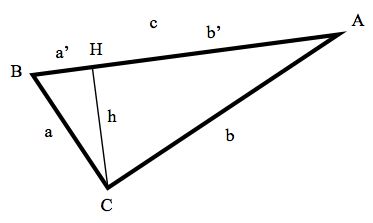
\includegraphics[width=\linewidth]{triangle-rect-intro}	}
%
%
%%%%%%%%%%%%%%%%%%%%%%%%%%%%%%%%%%%%%%%%%%%%%%%%%%%%%%%%%%%%%%%%%%
%
%
%\question
%\exonly{
%\FR{
%Soit le rectangle $ABCD$ et les deux triangles rectangles (en $E$) $BCE$ et $BEA$.
%
%Calculer $BE$, si $AD=12$ et $AB=5$.
%}}
%
%\exonly{\includegraphics*[width=\linewidth]{ch3-ex2}}
%
%\solonly{$BR=\frac{60}{13}\approx \num{4.62}$}
%
%%%%%%%%%%%%%%%%%%%%%%%%%%%%%%%%%%%%%%%%%%%%%%%%%%%%%%%%%%%%%%%%%%
%
%\question
%\exonly{
%\FR{
%Soit $ABC$ un triangle rectangle en $C$. 
%
%Exprimer les trois hauteurs du triangle en fonction de ses côtés $a$ et $b$.
%}
%}
%\solonly{$h_A=b$ \quad $h_B=c$ \quad $h_C=\dfrac{ab}{\sqrt{a^2 + b^2}}$}
%
%%%%%%%%%%%%%%%%%%%%%%%%%%%%%%%%%%%%%%%%%%%%%%%%%%%%%%%%%%%%%%%%%%
%
%\question
%\exonly{ $AF = AB = BC = CD = DE = 1$
%
%\FR{Calculer FE.}
%}
%
%
%\exonly{\includegraphics*[width=0.6\linewidth]{ch3-ex4}}
%\solonly{$FE=\sqrt{5}$}
%
%%%%%%%%%%%%%%%%%%%%%%%%%%%%%%%%%%%%%%%%%%%%%%%%%%%%%%%%%%%%%%%%%%
%\columnbreak
%
%
%\question
%\exonly{
%\FR{ 
%Calculer $x$ en fonction de $a$.} 
%}
%
%\exonly{\includegraphics*[width=\linewidth]{ch3-ex5}}
%
%\solonly{$x=\sqrt{8}\cdot a = 2 \cdot \sqrt{2} \cdot a$ }
%
%
%%%%%%%%%%%%%%%%%%%%%%%%%%%%%%%%%%%%%%%%%%%%%%%%%%%%%%%%%%%%%%%%%%
%
%\question 
%\exonly{
%\FR{
%Dans un cercle de rayon $7,3$ cm on trace deux cordes parallèles de longueur $9,6$ cm et $11,0$ cm.
%
%Calculer la distance entre les cordes.
%
%\textbf{rappels~:  }la distance entre deux droites est mesurée perpendiculairement,une corde est un segment reliant deux points du cercle.
%}
%}
%\solonly{$d_1=\SI{10.3}{\centi\meter}$ \quad $d_2=\SI{0.7}{\centi\meter}$}
%
%
%%%%%%%%%%%%%%%%%%%%%%%%%%%%%%%%%%%%%%%%%%%%%%%%%%%%%%%%%%%%%%%%%%
%
%
%\question 
%\exonly{
%\FR{
%Le diamètre d'un cercle est prolongé d'une longueur a. Du point P ainsi obtenu on trace une tangente au cercle, le point de tangence est T. On mesure t = PT la longueur de la tangente.
%
%Calculer le diamètre du cercle}}
%
%\begin{parts}  
%\part 
%\exonly{
%\FR{dans le cas particulier a = 12 et t = 26}} 
%\solonly{$d\approx \num{44.33}$}
%
%\part \exonly{\FR{dans le cas général (en fonction de $a$ et $t$).}} 
%
%\solonly{$d=\dfrac{t^2-a^2}{a}$}
%\end{parts}
%
%
%%%%%%%%%%%%%%%%%%%%%%%%%%%%%%%%%%%%%%%%%%%%%%%%%%%%%%%%%%%%%%%%%%
%
%%\solonly{\columnbreak}
%
%
%\question 
%\exonly{
%\FR{
%Calculer la longueur du segment de tangente $AB$ pour des cercles de rayon $r = \SI{4}{\centi\meter}$ et $R = \SI{9}{\centi\meter}$ lorsque
%}}
%
%\begin{parts}
%\part 
%\exonly{
%\FR{
%	les centres des cercles sont distants de \SI{20}{\centi\meter} 
%}} 
%
%\solonly{$AB=\SI{19.36}{\centi\meter} $}
%
%\part 
%\exonly{
%\FR{
%	les cercles sont tangents.
%}}
%
%\solonly{$AB=\SI{12}{\centi\meter} $}
%\end{parts}
%
%\exonly{\includegraphics[width=\linewidth]{ch3-ex8}}
%
%%%%%%%%%%%%%%%%%%%%%%%%%%%%%%%%%%%%%%%%%%%%%%%%%%%%%%%%%%%%%%%%%%
%
%
%
%\question
%\exonly{
%\FR{
%Chaque poutre de cette charpente a une longueur de \SI{8}{\meter}.
%
%Calculer la hauteur du toit.
%}} 
%
%\solonly{$h=\SI{10.58}{\meter}$}
%
%\exonly{\includegraphics*[width=\linewidth]{ch3-ex9}}
%
%
%%%%%%%%%%%%%%%%%%%%%%%%%%%%%%%%%%%%%%%%%%%%%%%%%%%%%%%%%%%%%%%%%%
%
%
%
%\question
%\exonly{
%\FR{
%Calculer $x$ si $r=\SI{25}{\centi\meter}$ et $a = \SI{38}{\centi\meter}$.
%}}
%
%\solonly{$x=\SI{32.5}{\centi\meter}$}
%
%\exonly{\includegraphics*[scale=1]{ch3-ex10}}
%
%%%%%%%%%%%%%%%%%%%%%%%%%%%%%%%%%%%%%%%%%%%%%%%%%%%%%%%%%%%%%%%%%%
%
%\question
%\exonly{% Frommenwiler, ex 65 ch 1.2.1 pg 29
%\FR{
%Calculer $EB$ sachant que le rayon du cercle circonscrit  $MD=\SI{3}{\centi\meter}$, \\ $AD = \SI{4.7}{\centi\meter}$ et $EF = \SI{2.7}{\centi\meter}$.}}
%
%\exonly{\includegraphics*[scale=.6]{ch3-ex11}}
%\solonly{$EB=\SI{2.22}{\centi\meter}$}
%
%
%
%\end{multicols}
%\end{questions}


%%\subfile{../ch/5_2-Heron}
%\subsection{Héron, Triangle isocèle et équilatéral}
%%\DE{\subsection{TODO}}
%
%\begin{questions}
%\begin{multicols}{2}
%\question
%\exonlyFR{Calculer l'aire du triangle $ABC$ si:}
%
%\exonly{$AB=\SI{7}{\centi\meter}$, $BC=\SI{6}{\centi\meter}$ et $AC=\SI{8}{\centi\meter}$.}
%\solonly{$\SI{20.33}{\square\centi\meter}$}
%
%
%
%
%%%%%%%%%%%%%%%%%%%%%%%
%\question
%\exonlyFR{Calculer la hauteur issue du sommet $A$ du triangle $ABC$ si:}
%\exonlyDE{TODO}
%
%\exonly{$AB=\SI{7}{\centi\meter}$ , $BC=\SI{6}{\centi\meter}$ et $AC=\SI{8}{\centi\meter}$.}
%\solonly{$h\approx \SI{6.78}{\centi\meter}$}
%
%%%%%%%%%%%%%%%%%%%%%%%
%
%\question
%\exonlyFR{Étant données les mesures des côtés du trapèze $ABCD$, déterminer son aire.}
%\exonlyDE{TODO}
%
%\exonly{$AB=\SI{3}{\centi\meter}$, $BC=\SI{4}{\centi\meter}$, 
%
%$CD=\SI{8}{\centi\meter}$, $AD=\SI{2}{\centi\meter}$ 
%
%\includegraphics*[scale=.6]{ch5-ex1}
%}
%
%\solonly{$\SI{8.36}{\square\centi\meter}$}
%
%%%%%%%%%%%%%%%%%%%%%%%%%%%%%%%%%%%
%
%
%\question
%\exonlyFR{
%Calculer $\varphi$ en fonction de $\alpha$ dans le cas particulier où $\alpha$ = 36${}^\circ$ puis dans un cas quelconque.}
%\exonlyDE{TODO}
%
%\exonly{\includegraphics*[scale=.6]{ch4-ex1}}
%\solonly{$\varphi=18^{\circ}$ et $\varphi= \dfrac{\alpha}{2}$}
%
%%%%%%%%%%%%%%%%%%%%%%%%%%%%%%%%%%%%%%%
%
%
%
%\question 
%\exonlyFR{
%Calculer le rayon $r$ de chacun deux cercles en fonction de $a$~: le côté du carré ou du triangle équilatéral.}
%\exonlyDE{TODO}
%
%\exonly{\includegraphics*[scale=1]{ch4-ex2}}
%\solonly{$r=\dfrac{\sqrt{2}a}{2}$ et $r=\dfrac{\sqrt{3}a}{4}$}
%
%%%%%%%%%%%%%%%%%%%%%%%%%%%%%%%%%%%%%%%
%
%\columnbreak
%
%\question
%\exonlyFR{
%$ABC$ est un triangle isocèle avec pour base 
%$AC=\SI{42}{\milli\meter}$ et $AB=BC=\SI{29}{\milli\meter}$.
%
%Calculer son aire et ses trois hauteurs.
%}
%\exonlyDE{TODO}
%
%\solonly{$h_B=\SI{20}{\milli\meter}$, $h_C=\SI{28.97}{\milli\meter}$, 
%
%$h_A=\SI{28.97}{\milli\meter}$, $A=\SI{420}{\square\milli\meter}$}
%
%
%%%%%%%%%%%%%%%%%%%%%%%%%%%%%%%%%%%%%%%
%
%
%\question 
%\exonlyFR{
%Les triangles $BCE$ et $BAC$ sont isocèles (en $C$, respectivement $A$). $AB =\SI{6}{\centi\meter}$
%}
%\exonlyDE{TODO}
%
%\exonly{\includegraphics*[scale=.8]{ch4-ex4}}
%\begin{parts}
%\part \exonlyFR{Déterminer tous les angles dans la figure.} 
%\exonlyDE{TODO}
%\solonly{
%$\angle{FCB}=45^{\circ}$
%$\angle{EBC}=\num{67.5}^{\circ}$
%
%$\angle{ADC}=\num{67.5}^{\circ}$
%$\angle{ADF}=\num{112.5}^{\circ}$
%
%$\angle{FBA}=\num{22.5}^{\circ}$
%}
%
%\part \exonlyFR{Calculer $AC$, $BC$, $EC$, $AE$, $BE$, $FC$.} 
%\exonlyDE{TODO}
%
%\solonly{
%$AC=\SI{6}{\centi\meter}$
%$BC=\SI{8.49}{\centi\meter}$
%$EC=\SI{8.49}{\centi\meter}$
%$AE=\SI{2.49}{\centi\meter}$
%$BE=\SI{6.5}{\centi\meter}$
%
%$FC=\SI{7.84}{\centi\meter}$
%}
%
%\part \exonlyFR{Trouver deux triangles égaux puis déterminer $AD$, $CD$ et $FD$.} 
%\exonlyDE{TODO}
%\solonly{
%$AD=\SI{2.49}{\centi\meter}$
%$CD=\SI{6.5}{\centi\meter}$
%
%$FD=\SI{1.34}{\centi\meter}$
%
%}
%\end{parts}
%
%%%%%%%%%%%%%%%%%%%%%%%%%%%%%%%%%%%%%%%
%\end{multicols}
%
%\end{questions}
%
%
%\exnewpage
%\subfile{../ch/5_2-Angle-centre}
\exnewpage
\subsection{Angolo al centro}
%\DE{\subsection{TODO}}

\begin{questions}

\question
\exonly{Calcolare $\alpha$, $\beta$, $\gamma$ e $\delta$.}

%TODO : convert in TikZ
\exonly{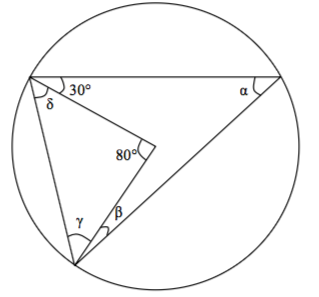
\includegraphics[width=0.5\linewidth]{aac-1}}

\solonly{$\alpha=40^{\circ}$, $\gamma=\delta=50^{\circ}$, $\beta=10^{\circ}$}

\question
\exonly{Calcolare $\alpha$, $\beta$, $\gamma$ e $\delta$.}

\exonly{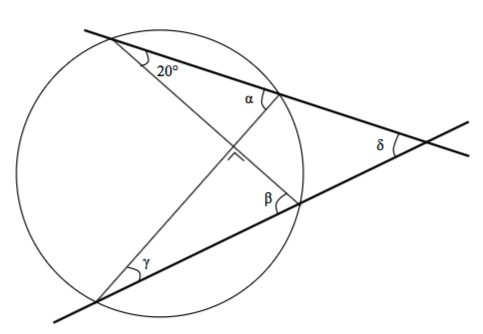
\includegraphics[width=0.6\linewidth]{aac-2}}

\solonly{$\gamma=20^{\circ}$, $\alpha=\beta=70^{\circ}$, $\delta=50^{\circ}$}

%\question
%\exonlyFR{Calculer les angles $\alpha$ et $\beta$ en sachant que $\gamma=80^{\circ}$ et $\delta=110^{\circ}$.}
%
%\exonly{\includegraphics[scale=0.8]{aac-3}}
%\solonly{$\alpha=100^{\circ}$, $\beta=70^{\circ}$}
%
%\question
%\exonlyFR{Un hélicoptère s'élève à la verticale d'un point A. 
%
%Sur le sol se trouvent trois points $A$, $B$ et $C$ alignés (dans cet ordre) tels que $AB = \SI{400}{\meter}$ et $BC = \SI{1}{\kilo\meter}$.
%
%L'hélicoptère voit les points $B$ et $C$ sous un angle de $30^\circ$.
%}
%
%\begin{parts}
%\part
%\exonlyFR{Faire un croquis de la situation.}
%
%\part
%\exonly{Dessiner l'ensemble des points $H'$ tels que $\angle{BH'C}=30^{\circ}$}
%
%\part
%\exonly{Calculer l'altitude de l'hélicoptère}
%\solonly{$h_1=\SI{430}{\meter}$, $h_2=\SI{1300}{\meter}$}
%\end{parts}




\end{questions}


%%\subfile{../ch/5_2-Droites-rem-cercles}
%\subsection{Droites remarquables, cercle inscrit et circonscrit}
%%\DE{\subsection{TODO}}
%
%\begin{questions}
%\begin{multicols}{2}
%
%\question
%\exonlyFR{
%Soit $ABC$ un triangle avec $a = 8$, $b = 9$ et $c = 14$. Calculer les rayons des cercles inscrit et circonscrit au triangle, son aire, la longueur des trois hauteurs et les trois angles du triangle.}
%\solonly{
%$r\approx\num{2.17}$ , $R\approx \num{7.48}$, $A\approx \num{33.67}$
%
%$h_A\approx \num{8.42}$, $h_B\approx \num{7.48}$, $h_C \approx \num{4.81}$
%}
%
%
%
%\question
%\exonlyFR{
%Soit $ABC$ un triangle rectangle en $C$ avec $a = 8$ et $b = 15$.  Calculer les rayons des cercles inscrit et circonscrit au triangle, son aire, la longueur des trois hauteurs et les trois angles du triangle.}
%\solonly{
%$r=3$ , $R=8.5$, $A=60$
%
%$h_A=b=15$, $h_B=a=8$, $h_C \approx \num{7.06}$
%}
%
%
%
%\question
%\exonly{
%Calculer les rayons des cercles inscrit et circonscrit à un triangle équilatéral de côté $a$.
%}
%\solonly{
%$r=\dfrac{\sqrt{3}}{6}a$ , $R=\dfrac{3 \sqrt{3}}{3}$, $A=\dfrac{\sqrt{3}}{4}a^2$
%}
%
%
%\question
%\exonly{
%Calculer les rayons des deux cercles inscrits dans un triangle isocèle de hauteur $h = 12$ cm et de base 10 cm.
%
%Le petit cercle est inscrit entre les deux côtés du triangle et le cercle inscrit au triangle.
%}
%\exonly{
%\includegraphics*[scale=1.3]{ch6-ex4}
%}
%
%\solonly{$r\approx \num{1.48}$, $R\approx 3,\!\overline{3}$}
%
%\todo[inline]{Ex sur les droites remarquables??}
%
%\end{multicols}
%\end{questions}
%
%\subsection{Triangolo rettangolo}
%\DE{\subsection{TODO}}


%\subsection{Triangolo rettangolo}
%\begin{questions}
%
%%%%%%%%%%%%%%%%%%%%%%%%%%%%%%%%%%%%%%%%%%%%%%%%%%%%%%%%%%%%%%%%%%%%%%%%%
%
%\question
%\exonly{ %Borgeaud 2.7.1. a)
%
%Calcolare i lati e gli angoli mancanti del triangolo qui sotto:
%}
%
%\ifprintanswers   \else     
%\begin{tikzpicture}[scale=1.3]
%\tkzInit[xmin=-1,xmax=5,ymin=-5,ymax=0.5]
%\tkzClip
%\tkzDefPoint(0,0){A}
%\tkzDefShiftPoint[A](-90:4.1){B}
%\tkzDefShiftPoint[B](0:1.9){C}
%\tkzDrawPolygon(A,B,C) 
%\tkzLabelPoints[above](A)
%\tkzLabelPoints[below](B,C)
%\tkzLabelSegment[above right](C,A){$b$}
%\tkzLabelSegment[below](C,B){\SI{19}{\meter}}
%\tkzLabelSegment[left](A,B){\SI{41}{\meter}}
%\tkzDefLine[orthogonal=through B](C,A) \tkzGetPoint{h1}
%\tkzInterLL(C,A)(B,h1) \tkzGetPoint{H}
%\tkzDrawSegment(B,H)
%\tkzLabelSegment[above left](H,B){$h$}
%\tkzMarkRightAngle(B,H,A)
%\tkzMarkRightAngle(C,B,A)
%%\tkzLabelAngle[pos=0.7](A,C,B){$\gamma$}
%%\tkzMarkAngle[arc=l,size=.5 cm](A,C,B)
%%\tkzLabelAngle[pos=0.7](C,B,A){$\beta$}
%%\tkzMarkAngle[arc=l,size=.5 cm](C,B,A)
%%
%%\tkzLabelAngle[pos=0.7](C,A,B){$\alpha$}
%%\tkzMarkAngle[arc=l,size=.5 cm](B,A,C)
%\end{tikzpicture}
%\fi
%
%\solonly{$b=\SI{45.19}{\meter}$ \quad $\angle BCA=\ang{65.14}$  \\ $\angle CAB= \ang{24.86}$  \quad $h=\SI{17.24}{\meter}$
%}
%
%%%%%%%%%%%%%%%%%%%%%%%%%%%%%%%%%%%%%%%%%%%%%%%%%%%%%%%%%%%%%%%%%
%
%\question
%\exonly{%Borgeaud 2.7.1. b)
%Calcolare i lati e gli angoli mancanti del triangolo qui sotto:
%
%\ifprintanswers   \else     
%\begin{tikzpicture}[scale=1.5]
%\tkzDefPoint(0,0){C}
%\tkzDefShiftPoint[C](-90:4.1){A}
%\tkzDefShiftPoint[C](0:1.9){B}
%\tkzDrawPolygon(A,B,C) 
%\tkzLabelPoints[above](C,B)
%\tkzLabelPoints[below](A)
%\tkzLabelSegment[left](C,A){$b$}
%\tkzLabelSegment[above](C,B){$a$}
%\tkzLabelSegment[right](A,B){\SI{105}{\meter}}
%\tkzLabelAngle[pos=1](B,A,C){$\ang{38}$}
%\tkzMarkAngle[arc=l,size=.5 cm](B,A,C)
%\tkzMarkRightAngle(B,C,A)
%\end{tikzpicture}
%\fi
%
%\solonly{$b=\SI{82.74}{\meter}$  $\angle CBA=\ang{52}$  \\ $a=\SI{64.64}{\meter}$
%}
%
%\exnewpage
%%%%%%%%%%%%%%%%%%%%%%%%%%%%%%%%%%%%%%%%%%%%%%%%%%%%%%%%%%%%%%%%%
%\question
%\exonly{ %Borgeaud 2.7.1. c)
%Calcolare i lati e gli angoli mancanti del triangolo qui sotto:
%
%
%\begin{tikzpicture}[scale=1.5]
%\tkzDefPoint(0,0){A}
%\tkzDefShiftPoint[A](-90:3){B}
%\tkzDefShiftPoint[B](0:4){C}
%\tkzDrawPolygon(A,B,C) 
%\tkzLabelPoints[below](C,B)
%\tkzLabelPoints[above](A)
%\tkzLabelSegment[above right](C,A){$b$}
%\tkzLabelSegment[below](C,B){\SI{30}{\meter}}
%\tkzLabelSegment[left](A,B){\SI{25}{\meter}}
%\tkzMarkRightAngle(C,B,A)
%\end{tikzpicture}
%}
%
%\solonly{$b=\SI{39.05}{\meter}$  $\angle BCA=\ang{39.81}$  \\ $\angle BAC=\ang{50.19}$
%}
%%%%%%%%%%%%%%%%%%%%%%%%%%%%%%%%%%%%%%%%%%%%%%%%%%%%%%%%%%%%%%%%%
%
%\question
%\exonly{%Borgeaud 2.7.1. d)
%Calcolare i lati e gli angoli mancanti del triangolo qui sotto:
%
%\begin{tikzpicture}[scale=0.8]
%\tkzDefPoint(0,0){A}
%\tkzDefShiftPoint[A](-90:3){B}
%\tkzDefShiftPoint[B](0:8){C}
%\tkzDrawPolygon(A,B,C) 
%\tkzLabelPoints[below](C,B)
%\tkzLabelPoints[above](A)
%\tkzLabelSegment[above right](C,A){\SI{50}{\meter}}
%\tkzLabelSegment[below](C,B){$a$}
%\tkzLabelSegment[left](A,B){$c$}
%\tkzMarkRightAngle(C,B,A)
%\tkzLabelAngle[pos=1.1](B,A,C){\footnotesize $1,2^{rad}$}
%\tkzMarkAngle[arc=l,size=.5 cm](B,A,C)
%\end{tikzpicture}
%
%}
%
%\solonly{$a=\SI{46.6}{\meter}$  $\angle BCA=\ang{21.25}$  \\ $c=\SI{18.12}{\meter}$
%}
%%%%%%%%%%%%%%%%%%%%%%%%%%%%%%%%%%%%%%%%%%%%%%%%%%%%%%%%%%%%%%%%%
%
%\question
%\exonly{%Borgeaud 2.7.4
%
%
%Qual'é l'altezza di una torre che proietta al suolo un ombra di \SI{96}{\metre} quando il sole forma un angolo \ang{52.5}  di con l'orizzonte?
%
%}
%\solonly{$\SI{125.11}{\meter}$}
%
%%%%%%%%%%%%%%%%%%%%%%%%%%%%%%%%%%%%%%%%%%%%%%%%%%%%%%%%%%%%%%%%%
%
%\question
%\exonly{%Borgeaud 2.7.5
%
%Determinare l'angolo formato dai raggi di sole e l'orizzonte se  se l'ombra di un palo vale  $\num{1.5}$ la sua altezza?
%
%%Quale angolo tra i raggi di soloe e l'orizzonte se l'ombra di un palo vale  $\num{1.5}$ la sua altezza?
%}
%
%\solonly{\ang{33.69}}
%
%%%%%%%%%%%%%%%%%%%%%%%%%%%%%%%%%%%%%%%%%%%%%%%%%%%%%%%%%%%%%%%%%
%
%%\question
%%\exonly{%Borgeaud 2.7.6
%%\FR{
%%Un mur de \SI{7.5}{\meter} de haut est à $5$ m d'une maison. Quelle serait la longueur la plus courte d'une échelle qui, partant du sol, puisse juste s'appuyer sur le haut du mur et atteindre une fenêtre située à \SI{10.2}{\meter} du sol?
%%}
%%\DE{}
%%}
%%
%%\solonly{\SI{21.47}{\meter}}
%%%%%%%%%%%%%%%%%%%%%%%%%%%%%%%%%%%%%%%%%%%%%%%%%%%%%%%%%%%%%%%%%%
%
%
%
%
%\end{questions}


\exnewpage
\subsection{Triangoli qualunque}

\begin{questions}

%%%%%%%%%%%%%%%%%%%%%%%%%%%%%%%%%%%%%%%%%%%%%%%%%%%%%%%%%%%%%%%%%%%%%%%%


\question
\exonly{
	Calcolare l'area dei triangoli qui sotto nelle situazioni date:
%	Calculer l'aire du triangle ci-dessous pour le situations suivantes:
}

\ifprintanswers   \else     
%\begin{adjustbox}{width=\linewidth}
\begin{tikzpicture}%[every node/.style={opacity=1, black, above left}] 
\path (0,0) coordinate (A)  node[left] {$A$};
\path (5,0) coordinate (B) node[right] {$B$};
\path (3,2) coordinate (C) node[above] {$C$};
\path (A) -- (B) node[midway,below] {$c$};
\path (B) -- (C) node[midway,above] {$a$};
\path (C) -- (A) node[midway,above] {$b$};
%\path ($(A)!0.5!(B)$) node [below] {$c$} ;
%\node at ($(A)!0.5!(B)$) [below] {$c$}  ;
%\node at ($(A)!0.5!(C)$) [above ] {$b$}  ;
%\node at ($(C)!0.5!(B)$) [above] {$a$}  ;
\draw (A)--(B)--(C) --cycle;
\path 
pic[pic text=$\alpha$,draw,angle eccentricity=1.5] {angle=B--A--C}
pic[pic text=$\beta$,draw,angle eccentricity=1.5] {angle=C--B--A}
pic[pic text=$\gamma$,draw,angle eccentricity=1.5] {angle=A--C--B}
;

\end{tikzpicture}
\fi

\begin{parts}
\part \exonly{$\alpha=\ang{40}$, $b=\SI{38}{\meter}$, $c=\SI{25}{\meter}$}
\solonly{\SI{305.32}{\square\meter}}

\part
\exonly{$\alpha =\ang{31}$, $\gamma=\ang{40}$, $a=\SI{53}{\meter}$}
\solonly{\SI{1657.47}{\square\meter}}

\end{parts}


%%%%%%%%%%%%%%%%%%%%%%%%%

\question
\exonly{
	Calcolare $\alpha$, $\beta$ e $\gamma$.
	}


\ifprintanswers   \else 
%\begin{tikzpicture}[scale=0.7]
%\tkzDefPoint(0,0){B}
%\tkzDefShiftPoint[B](35:5){C}
%\tkzDefShiftPoint[B](100:6){A}
%\tkzDrawPolygon(A,B,C) 
%\tkzLabelPoints[below](C,B)
%\tkzLabelPoints[above](A)
%\tkzLabelSegment[below right](C,B){$\SI{5}{\meter}$}
%\tkzLabelSegment[left](A,B){$\SI{7}{\meter}$}
%\tkzLabelSegment[above right](A,C){$\SI{6}{\meter}$}
%\tkzLabelAngle[pos=1.2](B,A,C){$\alpha$}
%\tkzMarkAngle[arc=l,size=.8 cm](B,A,C)
%\tkzLabelAngle[pos=-1.2](B,C,A){$\gamma$}
%\tkzMarkAngle[arc=l,size=.8 cm](A,C,B)
%\tkzLabelAngle[pos=0.8](A,B,C){$\beta$}
%\tkzMarkAngle[arc=l,size=.5 cm](C,B,A)
%\end{tikzpicture}


\begin{tikzpicture}[scale=0.7]
\coordinate[label=below :$B$]  (B) at (0,0);
\coordinate[label= right:$C$]  (C) at (35:5);
\coordinate[label=above:$A$]  (A) at (100:6);
\draw (A) -- node[midway, left] {$\SI{7}{\meter}$} (B) --node[midway, below right] {$\SI{5}{\meter}$} (C) --node[midway, above right] {$\SI{6}{\meter}$} cycle;
\path 
pic[pic text=$\alpha$,draw,angle eccentricity=1.5] {angle=B--A--C}
pic[pic text=$\beta$,draw,angle eccentricity=1.5] {angle=C--B--A}
pic[pic text=$\gamma$,draw,angle eccentricity=1.5] {angle=A--C--B};
\end{tikzpicture}
\fi

\solonly{$\alpha \approx \num{44.42}^{\circ}$, $\beta \approx \num{57.12}^{\circ}$, $\gamma \approx \num{78.46}^{\circ}$}

%%%%%%%%%%%%%%%%%%%%%%%%%%%%%%%%%%%%%%%%%%%%%%%%%%%%%%%%%%%%%%%
%
%\question
%\exonly{
%\FR{
%Un ballon $S$ et deux observateurs $A$ et $B$ se trouvent dans le même plan vertical.
%On a mesuré $AB=\SI{400}{\meter}$, $\angle BAS = \ang{55}$ et $\angle ABS = \ang{45}$.
%
%Calculer la hauteur $h$ du ballon.
%}
%\DE{
%
%}}
%
%\solonly{
%$h=\SI{235.27}{\meter}$
%}
%
%


%%%%%%%%%%%%%%%%%%%%%%%%%%%%%%%%%%%%%%%%%%%%%%%%%%%%%%%%%%%%%%%

\question
\exonly{
Calcolare $c$, $\beta$ e $\gamma$.}

\ifprintanswers   \else  
%\begin{tikzpicture}[scale=0.7]
%\tkzDefPoint(0,0){B}
%\tkzDefShiftPoint[B](0:5){C}
%\tkzDefShiftPoint[B](76:6){A}
%\tkzDrawPolygon(A,B,C) 
%\tkzLabelPoints[below](C,B)
%\tkzLabelPoints[above](A)
%\tkzLabelSegment[below](C,B){$\SI{5}{\meter}$}
%\tkzLabelSegment[left](A,B){$c$}
%\tkzLabelSegment[above right](A,C){$\SI{7}{\meter}$}
%\tkzLabelAngle[pos=1.2](B,A,C){$35^{\circ}$}
%\tkzMarkAngle[arc=l,size=.8 cm](B,A,C)
%\tkzLabelAngle[pos=1.2](B,C,A){$\gamma$}
%\tkzMarkAngle[arc=l,size=.8 cm](A,C,B)
%\tkzLabelAngle[pos=0.8](A,B,C){$\beta$}
%\tkzMarkAngle[arc=l,size=.5 cm](C,B,A)
%\end{tikzpicture}

\begin{tikzpicture}[scale=0.7]
\coordinate[label=below :$B$]  (B) at (0,0);
\coordinate[label= right:$C$]  (C) at (0:5);
\coordinate[label=above:$A$]  (A) at (76:6);
\draw (A) -- node[midway, left] {$c$} (B) --node[midway, below ] {$\SI{5}{\meter}$} (C) --node[midway, above right] {$\SI{7}{\meter}$} cycle;
\path 
pic[pic text=$35\degree$,draw,angle eccentricity=1.5] {angle=B--A--C}
pic[pic text=$\beta$,draw,angle eccentricity=1.5] {angle=C--B--A}
pic[pic text=$\gamma$,draw,angle eccentricity=1.5] {angle=A--C--B};
\end{tikzpicture}
\fi

\solonly{$\beta_1 \approx \num{53.42}^{\circ}$, $\gamma_1 \approx \num{91.58}^{\circ}$, $c_1\approx \SI{8.71}{\meter}$}

\solonly{$\beta_2 \approx \num{126.58}^{\circ}$, $\gamma_2 \approx \num{18.42}^{\circ}$, $c_2\approx \SI{2.75}{\meter}$}

%%%%%%%%%%%%%%%%%%%%%%%%%%%%%%%%%%%%%%%%%%%%%%%%%%%%%%%%%%%%%%%%%%%%%%%%%
\exnewpage
\question
\exonly{
Calcolare $c$, $\alpha$, $\beta$ e $\gamma$ se l'area del triangolo é di $\SI{12}{\square\meter}$.
}

\exonly{
%\begin{tikzpicture}[scale=0.7]
%\tkzDefPoint(0,0){B}
%\tkzDefShiftPoint[B](0:3){C}
%\tkzDefShiftPoint[B](64:5){A}
%\tkzDrawPolygon(A,B,C) 
%\tkzLabelPoints[below](C,B)
%\tkzLabelPoints[above](A)
%\tkzLabelSegment[below](C,B){$\SI{6}{\meter}$} %CB
%\tkzLabelSegment[left](A,B){$c$}  % AB
%\tkzLabelSegment[above right](A,C){$\SI{5}{\meter}$} %AC
%\tkzLabelAngle[pos=1.2](B,A,C){$\alpha$} %alpha
%\tkzMarkAngle[arc=l,size=.8 cm](B,A,C)
%\tkzLabelAngle[pos=1.2](B,C,A){$\gamma$} %gamma
%\tkzMarkAngle[arc=l,size=.8 cm](A,C,B)
%\tkzLabelAngle[pos=0.8](A,B,C){$\beta$} %beta
%\tkzMarkAngle[arc=l,size=.5 cm](C,B,A)
%\end{tikzpicture}
\begin{tikzpicture}[scale=0.8]
\coordinate[label=below :$B$]  (B) at (0,0);
\coordinate[label= right:$C$]  (C) at (0:3);
\coordinate[label=above:$A$]  (A) at (64:5);
\draw (A) -- node[midway, left] {$c$} (B) --node[midway, below ] {$\SI{6}{\meter}$} (C) --node[midway, above right] {$\SI{5}{\meter}$} cycle;
\path 
pic[pic text=$\alpha$,draw,angle eccentricity=1.5] {angle=B--A--C}
pic[pic text=$\beta$,draw,angle eccentricity=1.5] {angle=C--B--A}
pic[pic text=$\gamma$,draw,angle eccentricity=1.5] {angle=A--C--B};
\end{tikzpicture}
}

\solonly{$\alpha_1 \approx \ang{73.74}$, $\beta_1 \approx \ang{53.13}$ \\$\gamma_1 \approx \ang{53.13}$, $c_1\approx \SI{5}{\meter}$}

\solonly{$\alpha_2 \approx \ang{29.16}$, $\beta_2 \approx \ang{23.97}$ \\ $\gamma_2 \approx \ang{126.87}$, $c_2\approx \SI{9.85}{\meter}$}


\question
\exonly{
Per stimare l'altezza di una montagna per triangolazione un osservatore misura l'angolo di elevazione $\alpha=\ang{25}$ (angolo tra l'orizzontale e la cima della montagna). In seguito, spostandosi sullo sullo stesso piano, si avvicina  percorre $d=\SI{1000}{\meter}$ in direzione della montagna  e misura di nuovo l'angolo di elevazione che ora é di $\beta=\ang{38}$.

Stimare l'altezza $h$ della montagna rispetto al piano sul quali si trova l'osservatore.

}

\solonly{$h=\SI{1156.65}{\meter}$}
%%%%%%%%%%%%%%%%%%%%%%%%%%%%%%%%%%%%%%%%%%%%%%%%%%%%%%%%%%%%%%%
%\question
%\exonly{\FR{
%Dans un triangle quelconque, on connait les trois côtés $a=\SI{10}{\meter}$, $b=\SI{4}{\meter}$ et $c=\sqrt{52} \:\SI{}{\meter}$.
%
%Calculer la longueur $AM$ de la médiane issue de $A$.
%}}
%
%\solonly{$AM=\SI{3}{\meter}$}

%%%%%%%%%%%%%%%%%%%%%%%%%%%%%%%%%%%%%%%%%%%%%%%%%%%%%%%%%%%%%%%

\question
\exonly{

La torre di Pisa ha un'inclinazione di \ang{10;15;} rispetto alla verticale.
Quando é inclinata verso il sole, i cui raggi formano un angolo di \ang{33} con l'orizzonte, l'ombra della torre misura \SI{74.9}{\meter}.

Qual'era l'altezza originale della torre? 


}

\solonly{$h=\SI{56}{\meter}$
}

%%%%%%%%%%%%%%%%%%%%%%%%%%%%%%%%%%%%%%%%%%%%%%%%%%%%%%%%%%%%%%%
%
%\question
%\exonly{
%\FR{
%Pour mesurer la hauteur d'une montagne par triangulation, un observateur mesure l'angle d'élévation $\alpha=\ang{25}$ de celle--ci (angle sous lequel il voit le sommet de la montagne). Il se rapproche ensuite de la montagne d'une distance $d=\SI{1000}{\meter}$ et mesure à nouveau l'angle d'élévation $\beta=\ang{38}$. 
%
%Calculer la hauteur $h$ de la montagne.
%}
%\DE{
%
%}}

\solonly{$h=\SI{1156.65}{\meter}$
}

\exnewpage
\subsection{Poligoni e cerchi}


\begin{questions}
	
	%%%%%%%%%%%%%%%%%%%%%%%%%%%%%%%%%%%%%%%%%%%%%%%%%%%%%%%%%%%%%%%%%%%%%%%%
	
	
	\question
	\ifprintanswers \else
		Calcolare la lunghezza $L_1$.% e $L_2$.
		
		\begin{minipage}{0.4\textwidth}
%			\begin{tikzpicture}%[scale=.8]
%			\tkzDefPoint(0,0){O}
%			\tkzDefShiftPoint[O](0:2.5){A}
%			\tkzDefShiftPoint[O](120:2.5){B}
%			\tkzDrawCircle[R,dashed](O,2,5 cm)
%			\tkzDrawSegments(O,A O,B)
%			\tkzLabelSegment[below](O,A){$r=2,5$ m}
%			\tkzDrawArc[ultra thick,color=black](O,A)(B)
%			\tkzLabelAngle[pos=3](A,O,B){$L_1$}
%			\tkzMarkAngle[arc=l,size=0.5 cm,](A,O,B)
%			\tkzLabelAngle[pos=0.8,circle](A,O,B){$120^\circ$}
%			\tkzDrawSegments(O,A O,B)
%			\end{tikzpicture}
			\begin{tikzpicture}
			\coordinate (O) at (0,0);
			\coordinate (B) at (120:2.5);
			\coordinate (A) at (0:2.5);
			\draw (A) -- node[midway, below] {$r=\SI{2.5}{\meter}$} (O) -- (B);
			\path 
			pic[pic text=$120\degree$,draw,angle eccentricity=1.5] {angle=A--O--B};
			\draw[dashed] (O) circle (2.5);
			\draw[very thick] (A) arc (0:120:2.5) node[midway, above] {$L_1$} ;
			\end{tikzpicture}
			
		
		\end{minipage}
		
		%\begin{minipage}{0.4\textwidth}
		%\begin{tikzpicture}%[scale=.8]
		%\tkzDefPoint(0,0){O}
		%\tkzDefShiftPoint[O](0:2.5){A}
		%\tkzDefShiftPoint[O](300:2.5){B}
		%\tkzDrawCircle[R,dashed](O,2,5 cm)
		%\tkzDrawSegments(O,A O,B)
		%\tkzLabelSegment[below](O,A){$r=5$ m}
		%\tkzDrawArc[ultra thick,color=black](O,A)(B)
		%\tkzLabelAngle[pos=-3](A,O,B){$L_2$}
		%\tkzMarkAngle[arc=l,size=0.5 cm,](A,O,B)
		%\tkzLabelAngle[pos=-0.8,circle](A,O,B){$300^\circ$}
		%\tkzDrawSegments(O,A O,B)
		%\end{tikzpicture}
		%\end{minipage}
	\fi
	
	
	\solonly{$L_1=\SI{5.24}{\meter}$ }%\qquad $L_2=\SI{26.18}{\meter}$}
	
	%%%%%%%%%%%%%%%%%%%%%%%%%%%%%%%%%%%%%%%%%%%%%%%%%%%%%%%%
	%\question
	%\exonly{
	%\FR{
	%Si la latitude augmente de \ang{;1;}, alors la distance parcourue sur la surface de la terre se nomme le mille marin. Sachant que la terre a un diamètre approximatif de \SI{12800}{\kilo\meter}, calculer cette distance en \SI{}{\kilo\meter}.
	%}
	%
	%Se la latitudine aumenta di \ang{;1;} la distanza 
	%}
	%
	%\solonly{\SI{1.861}{\kilo\meter}
	%
	%}
	
	%%%%%%%%%%%%%%%%%%%%%%%%%%%%%%%%%%%%%%%%%%%%%%%%%%%%%%%%
	
	
	\question
	\exonly{
		L'estremità di un pendolo di \SI{60}{\centi\meter} descrive, oscillando, un arco di \SI{17}{\centi\meter}.
		
		Calcolare l'angolo percorso dal file del pendolo durante un oscillazione.
	}
	
	\solonly{ \ang{16.23}}
	
	
	%%%%%%%%%%%%%%%%%%%%%%%%%%%%%%%%%%%%%%%%%%%%%%%%%%%%%%%%
	
	%%%%%%%%%%%%%%%%%%%%%%%%%%%%%%%%%%%%%%%%%%%%%%%%%%%%%%%%%%%%%%%
	%\exonly{\columnbreak}
	\question
	\exonly{
		Calcolare la lunghezza della strada (le parti curve sono archi di cerchio).
		
	%	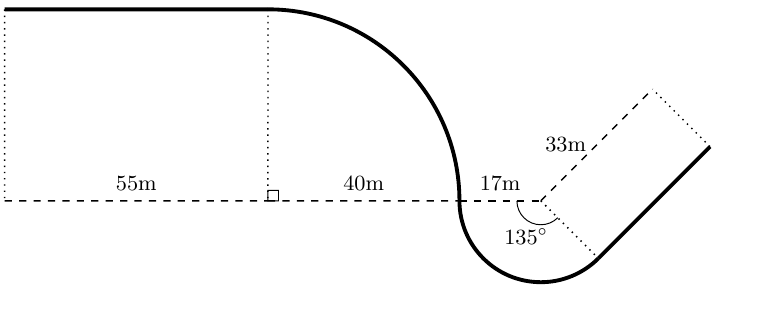
\includegraphics[scale=1]{es1-5-3}
		
		\begin{tikzpicture}[scale=0.7]
		\tkzDefPoint(0,0){O}
		\tkzDefPoint(-5.7,0){O1}
		\tkzDefShiftPoint[O](-1.7,0){P3}
		\tkzDefShiftPoint[P3](-4,4){P2}
		\tkzDefShiftPoint[P2](0,-4){P2a}
		\tkzDefShiftPoint[P2](-5.5,0){P1}
		\tkzDefShiftPoint[P1](0,-4){P1a}
		\tkzDefShiftPoint[O](-45:1.7){P4}
		\tkzDefShiftPoint[P4](45:3.3){P5}
		\tkzDefShiftPoint[P5](135:1.7){P5a}
		\tkzDrawSegments[ultra thick,color=black](P1,P2 P4,P5)
		\tkzDrawArc[ultra thick,color=black](O,P3)(P4)
		\tkzDrawArc[ultra thick,color=black](O1,P3)(P2)
		\tkzDrawSegments[dashed,color=black](P1a,P2a   P2a,P3 P3,O  O,P5a)
		\tkzDrawSegments[dotted,color=black](P1,P1a P2,P2a  O,P4  P5,P5a)
		\tkzLabelSegment(P1a,P2a){\footnotesize $55$m}
		\tkzLabelSegment(P3,P2a){\footnotesize  $40$m}
		\tkzLabelSegment(P3,O){\footnotesize  $17$m}
		\tkzLabelSegment[left](O,P5a){\footnotesize $33$m}
		\tkzMarkAngle[arc=l,size=0.5 cm,](P3,O,P4)
		\tkzLabelAngle[pos=-0.8,circle](P3,O,P4){\footnotesize  $135^\circ$}
		\tkzMarkRightAngle(P2,P2a,P3)
		\end{tikzpicture}
		%TODO diegno in tikz

	}
	
	\solonly{$\SI{190.89}{\meter}$}
	
	%%%%%%%%%%%%%%%%%%%%%%%%%%%%%%%%%%%%%%%%%%%%%%%%%%%%%%%%%%%%%%%
	%\exonly{\columnbreak}
	%\question
	%\exonly{
	%\FR{
	%Sur le schéma ci-dessous, en noir est représenté la plan d'une route. Calculer la longueur du virage. Le virage a un rayon de courbure de \SI{122}{\meter}.
	%}
	%\DE{}
	%
	%
	%
	%\begin{tikzpicture}%[scale=.8]
	%\tkzDefPoint(0,0){O}
	%\tkzDefShiftPoint[O](0,3){P2}
	%\tkzDefShiftPoint[P2](-3,0){P1}
	%\tkzDefShiftPoint[O](30:3){P3}
	%\tkzDefShiftPoint[P3](-60:2){P4}
	%\tkzDrawSegments[ultra thick,color=black](P1,P2 P3,P4)
	%\tkzDrawArc[ultra thick,color=black](O,P3)(P2)
	%\tkzInterLL(P1,P2)(P3,P4)  \tkzGetPoint{I}
	%\tkzDrawSegments[dashed,color=black](P2,I I,P4)
	%\tkzMarkAngle[arc=l,size=0.5 cm,](P3,I,P2)
	%\tkzLabelAngle[pos=0.8,circle](P2,I,P3){$240^\circ$}
	%%\tkzLabelSegment[left](O,P5a){$33$m}
	%%\tkzMarkAngle[arc=l,size=0.5 cm,](P3,O,P4)
	%%\tkzLabelAngle[pos=-0.8,circle](P3,O,P4){$135^\circ$}
	%%\tkzMarkRightAngle(P2,P2a,P3)
	%\end{tikzpicture}
	%}
	%
	%\solonly{$\SI{129.76}{\meter}$}
	%
	%
	%%%%%%%%%%%%%%%%%%%%%%%%%%%%%%%%%%%%%%%%%%%%%%%%%%%%%%%%%
	%\question
	%\exonly{
	%\FR{
	%Paris et Niamey, la capitale du Niger, sont sur le même méridien. Paris a une latitude de \ang{45;52;} et Niamey une latitude de \ang{13;31;}. Sachant que la terre a un diamètre approximatif de \SI{12800}{\kilo\meter}, calculer la distance entre les deux villes. Faire un croquis de la situation.
	%}
	%}
	%
	%\solonly{\SI{3613.53}{\kilo\meter}}
	%
	%
	%\question
	%\exonly{
	%\FR{
	%Calculer l'aire d'un secteur circulaire (de rayon \SI{11}{\centi\meter}) dont l'angle au centre mesure:
	%}
	%\DE{
	%
	%}}
	%
	%\begin{parts}
	%\part
	%\exonly{\ang{55}} \solonly{\SI{58.08}{\square\centi\meter}}
	%
	%\part
	%\exonly{$\dfrac{\pi}{5}$ \SI{}{\radian}} \solonly{\SI{38.01}{\square\centi\meter}}
	%
	%\end{parts}
	
	
	%%%%%%%%%%%%%%%%%%%%%%%%%%%%%%%%%%%%%%%%%%%%%%%%%%%%%%%%%%%%%%%%%%%%%%%%
	\question
	\exonly{
		I rettangoli  $R_1$, $R_2$, $R_3$ e $R_4$ hanno la stessa superficie.
		
		Calcolare l'area e il perimetro della figura.
		
		%TODO : convert in TikZ
		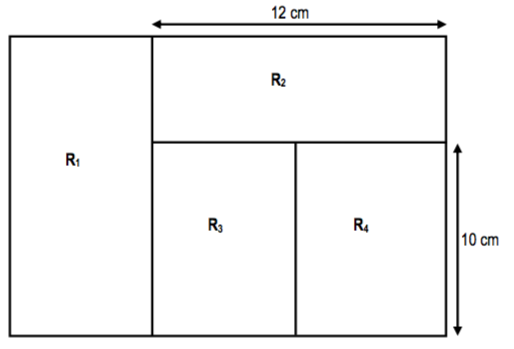
\includegraphics[width=0.5\linewidth]{surf-1}
	}
	
	\solonly{
		$A=\SI{240}{\square\centi\meter}$ \\
		$P=\SI{62}{\centi\metre}$
	}
	
	%%%%%%%%%%%%%%%%%%%%%%%%%%%%%%%%%%%%%%%%%%%%%%%%%%%%%%%%%%%%%%%%%%%%%%%%
	%
	%\question
	%\exonly{
	%\FR{
	%$ABCD$ est un rectangle et $M$ est le milieu de $CD$. L'aire du triangle $\Delta_2$ a $\SI{4}{\square\centi\meter}$ de plus que l'aire du triangle $\Delta_1$. Calculez l'aire du triangle grisé.
	%}
	%
	%\includegraphics[width=\linewidth]{surf-2}
	%}
	%
	%\solonly{
	%$\FR{A}\DE{F}=\SI{25.5}{\square\centi\meter}$
	%}
	%
	%%%%%%%%%%%%%%%%%%%%%%%%%%%%%%%%%%%%%%%%%%%%%%%%%%%%%%%%%%%%%%%%%%%%%%%%
	
	
	%\question
	%\exonly{
	%\FR{
	%On considère un parallélogramme $ABCD$. Son périmètre vaut $\SI{25.2}{\centi\meter}$ et le côté $AB$ est deux fois plus grand que le côté $BC$. La somme des longueurs des deux hauteurs de ce parallélogramme donne $\SI{12}{\centi\meter}$. Calculez la surface de ce parallélogramme.
	%}}
	%\solonly{
	%$\FR{A}\DE{F}=\SI{33.6}{\square\centi\meter}$
	%}
	%%%%%%%%%%%%%%%%%%%%%%%%%%%%%%%%%%%%%%%%%%%%%%%%%%%%%%%%%%%%%%%%%%%%%%%%
	
	%\question
	%\exonly{
	%\FR{
	%Le périmètre d’un losange vaut  $\SI{42}{\centi\meter}$. Le rayon du cercle inscrit à ce losange vaut  $\SI{3.2}{\centi\meter}$. Calculez l'aire du losange.
	%}}
	%\solonly{
	%$\FR{A}\DE{F}=\SI{67.2}{\square\centi\meter}$
	%}
	
	%%%%%%%%%%%%%%%%%%%%%%%%%%%%%%%%%%%%%%%%%%%%%%%%%%%%%%%%%%%%%%%%%%%%%%%%
\exnewpage
	\question
	\exonly{
		Calcolare l'area della superficie in grigio. 
		Il lato del quadrato misura $\SI{10}{\centi\meter}$.
		$A$ e $B$ sono i centri degli archi di cerchio.
		
		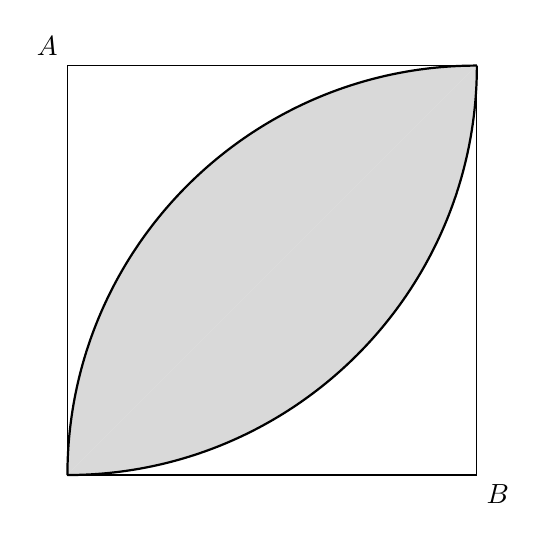
\begin{tikzpicture}[scale=1.3]
		\filldraw[gray!30] (4,0) arc (90:180:4) ;
		\filldraw[gray!30] (4,0) arc (0:-90:4);
		\draw (0,0) node[above left] {$A$} rectangle (4,-4) node[below right] {$B$};
		\draw[thick] (4,0) arc (90:180:4);
		\draw[thick] (4,0) arc (0:-90:4);
		\end{tikzpicture}
		%\includegraphics[width=0.6\linewidth]{surf-3}
	}
	
	
	\solonly{
		$A\approx\SI{57.08}{\square\centi\meter}$
	}
	
	%%%%%%%%%%%%%%%%%%%%%%%%%%%%%%%%%%%%%%%%%%%%%%%%%%%%%%%%%%%%%%%%%%%%%%%%
	%
	%\question 
	%\exonly{
	%\FR{Soient $C_1$ et $C_2$  deux cercles tangents en $B$. Le rayon $r_1$ mesure $\SI{4.5}{\centi\meter}$ et $\alpha= 60^{\circ}$. $t$ est la tangente commune aux deux cercles.}}
	%
	%\begin{parts}
	%\part
	%\exonly{\FR{
	%	Calculez le rayon $r_2$.
	%}} \solonly{$r_2=\SI{1.5}{\centi\meter}$}
	%
	%\part
	%\exonly{\FR{
	%	Calculez l'aire de la surface grisée.
	%}} \solonly{$A\approx\SI{2.64}{\square\centi\meter}$}
	%
	%\end{parts}
	%
	%\exonly{
	%\includegraphics[width=\linewidth]{surf-4}
	%}
	%
	
	%%%%%%%%%%%%%%%%%%%%%%%%%%%%%%%%%%%%%%%%%%%%%%%%%%%%%%%%%%%%%%%%%%%%%%%%
	
	\question 
	\exonly{
		Calcolare l'area della superficie in grigio.
		Il lato del quadrato misura $\SI{7}{\centi\meter}$.
		$A$ e $B$ sono i centri degli archi di cerchio.
	}
	
	\exonly{
		
		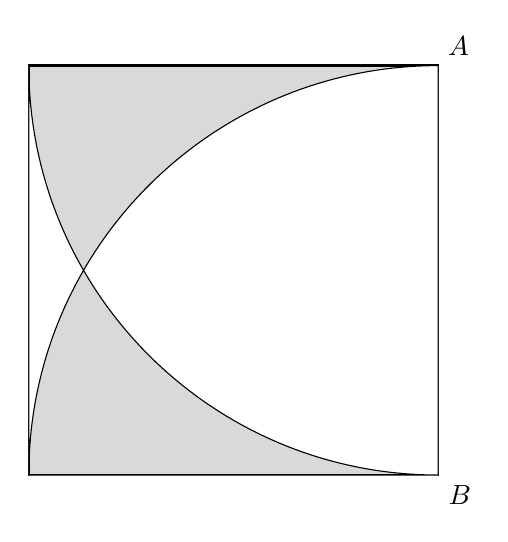
\begin{tikzpicture}[scale=1.3]
		\path (4,0) node[above right] {$A$} ;
		\filldraw[thick,draw=black,fill=gray!30] (0,0) rectangle (4,-4) node[below right] {$B$};
		
		\clip (0,0) rectangle (4,-4);
		\begin{scope}
		\filldraw[draw=black,fill=white,even odd rule] (0,0) rectangle (4,-4) (4,-4) circle (4) (4,0) circle (4) ;
		\end{scope}
		
		\end{tikzpicture}
		
		%\includegraphics[width=0.6\linewidth]{surf-5}
	}
	
	\solonly{
		$A\approx\SI{16.76}{\square\centi\meter}$
	}
	
	%%%%%%%%%%%%%%%%%%%%%%%%%%%%%%%%%%%%%%%%%%%%%%%%%%%%%%%%%%%%%%%%%%%%%%%%
	
	\question 
	\exonly{
		L'arco di cerchio (di centro $O$) qui sotto ha un angolo al centro di \ang{230}.
		La lunghezza della corda $AB$ é di $\SI{7}{\meter}$.
		
		Calcolare il raggio $R$ dell'arco di cerchio e l'altezza $H$.}
	
	\exonly{
		\begin{tikzpicture}[scale=0.8]
		\draw (0,0) node[above] {$O$} -- node[above, midway] {$R$} (15:4);
		\draw (-45:4) node[below] {$B$} arc (-45:225:4) node[below] {$A$};
		\draw (-45:4) --  + (0:2) -- +(180:8);
		\draw[dashed] (-45:4) ++(0:1.5) |- (0,4);
		\coordinate (A) at ({$(-45:4)+(0:1.5)$} |- {$(0,4)$});
		\draw[latex-latex, thick] (-45:4) ++(0:1.5) -- node[right,midway]{$H$}(A);
		
		\end{tikzpicture}
		
		
		%\includegraphics[width=\linewidth]{surf-6}
	}
	
	\solonly{
		$R\approx\SI{3.86}{\meter}$ , $H\approx\SI{5.49}{\meter}$
	}
	
	
\end{questions}



%%%%%%%%%%%%%%%%%%%%%%%%%%%%%%%%%%%%%%%%%%%%%%%%%%%%%%%%%%%%%%%

\end{questions}